\subsubsection{Prospetto Orario}
Di seguito è riportata la suddivisione oraria dei ruoli nel periodo di Analisi.




\begin{table}[H]	
	\begin{center}
	    \begin{tabular}{cccccccc}
			\rowcolor{greySWEight}
			\textcolor{white}{\textbf{Nome}} & \textcolor{white}{\textbf{Re}} & \textcolor{white}{\textbf{Am}} & \textcolor{white}{\textbf{An}} & \textcolor{white}{\textbf{Pj}} & \textcolor{white}{\textbf{Pr}} & \textcolor{white}{\textbf{Ve}} & \textcolor{white}{\textbf{Totale}}
			\\
			Bacco Alberto & & 5 & & & & 15 & 20 \\
			Caccaro Sebastiano & 15 & & 5 & & & & 20 \\
			Ciagola Damien & & & 15 & & & 5 & 20\\
			Corti Francesco & & & 15 & & & 5 & 20\\
			Isachi Gheorghe & & & 5 & & & 15 & 20\\
			Legrottagle Gionata & 5 & 15 & & & & & 20\\
			Magarotto Francesco & & & 15 & & & 5 & 20\\
			Muraro Enrico & & & 15 & & & 5 & 20\\
			\end{tabular}
	    \caption{Tabella della suddivisione oraria dei membri del gruppo nel periodo di Analisi} \label{tab:tabellaPersoneAnalisi} 
	\end{center}
\end{table}

La tabella della suddivisione oraria è rappresentata nel seguente grafico.
\begin{figure}[H]
	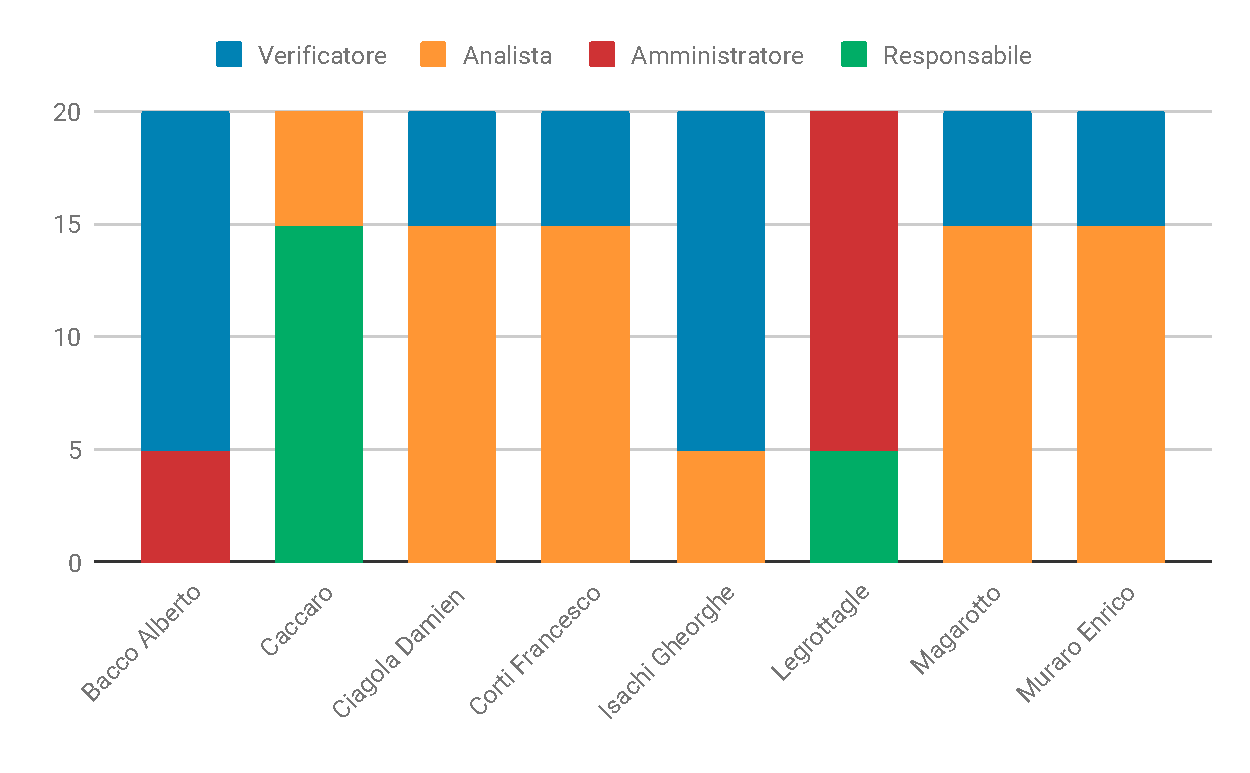
\includegraphics[width=1\linewidth]{Preventivo/grafici/AN1.pdf}
	\caption{Grafico della suddivisione oraria dei membri del gruppo nel periodo di Analisi}
\end{figure}

\subsubsection{Prospetto Economico}
Nella seguente tabella sono riportate le ore e i costi preventivati per ogni ruolo durante la fase di Analisi.


\begin{table}[H]	
	\begin{center}
	    \begin{tabular}{C{4cm}C{1cm}C{3,5cm}}
			\rowcolor{greySWEight}
			\textcolor{white}{\textbf{Ruolo}} & \textcolor{white}{\textbf{Ore}} & \textcolor{white}{\textbf{Costo}}
			\\
			Responsabile & 20 & \euro \space 600,00 \\
			Amministratore & 20 & \euro \space 400,00 \\
			Analista & 70 & \euro \space 1.750,00 \\
			Progettista &  & \\
			Programmatore &  & \\
			Verificatore & 50 & \euro \space 750,00 \\
			\textbf{Totale} & \textbf{160} & \textbf{\euro \space 3.500,00} \\
		\end{tabular}
	    \caption{Tabella della suddivisione oraria dei ruoli nel periodo di Analisi} \label{tab:tabellaRuoliAnalisi} 
	\end{center}
\end{table}


Si può avere una più chiara rappresentazione della distribuzione oraria dei ruoli nel seguente grafico.

\begin{figure}[H]
	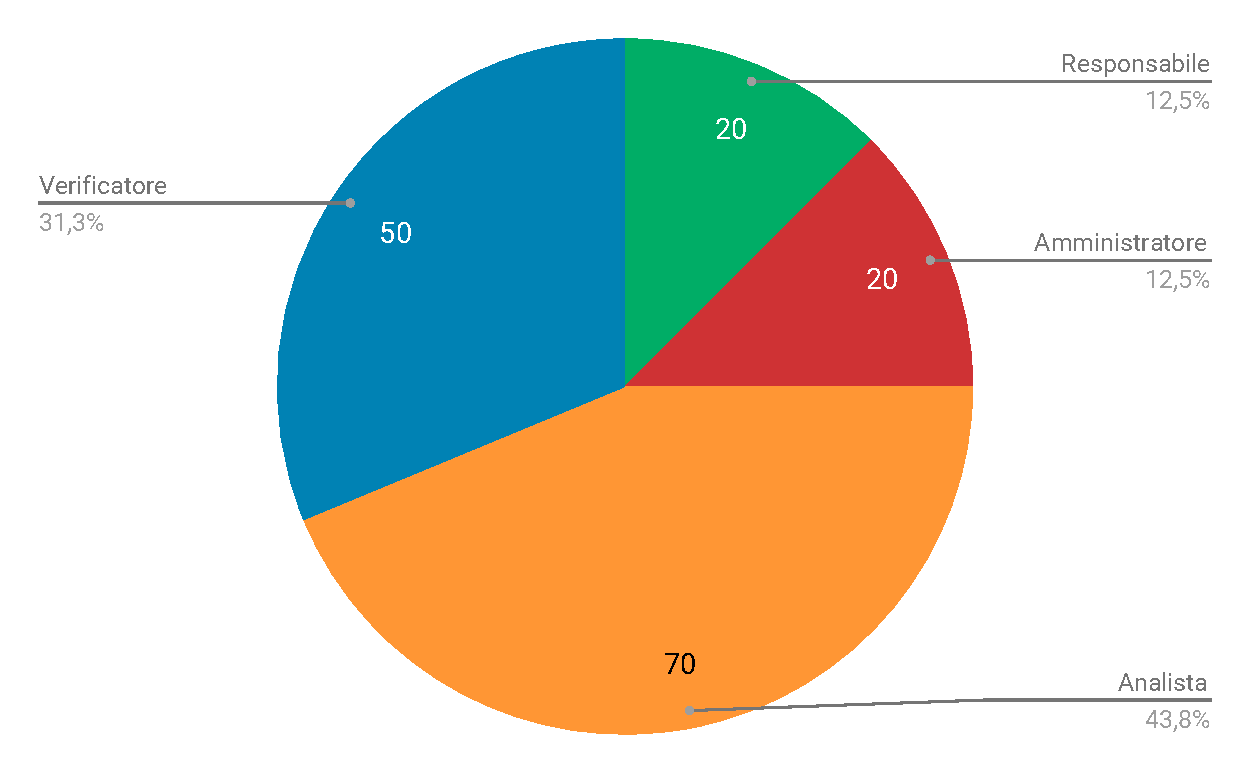
\includegraphics[width=1\linewidth]{Preventivo/grafici/AN2.pdf}
	\caption{Grafico della suddivisione oraria dei ruoli nel periodo di Analisi}
\end{figure}

